\appendix

\section{Auswertung Statistiken}
\label{app:statistik}
Alle Statistiken basieren auf dem Zeiterfassungsprogramm pTime (ptime.insode.ch), welches wir extra f�r dieses Projekt neu programmiert haben. Jeder Eintrag konnte minutenweise einem Modul (Algorithmus, Netzwerk, GUI, ...) und einer Aktivit�t (Design, Dokumentation, Meeting, ...) zugeordnet werden. Somit ist eine genaue Auswertung unserer T�tigkeiten m�glich und wir k�nnen die gewonnenen Erkenntnisse in die Planung der Diplomarbeit einfliessen lassen. Alle Daten der folgenden Statistiken sind vom 15. Juni 2005, 10:00 Uhr MEZ.



\subsection{Arbeits-Fortschritt}
Wochenweise aufgeteilt werden die aufsummierten Stunden der einzelnen Module visualisiert.
\begin{figure}[H]
\centering
%\frame{
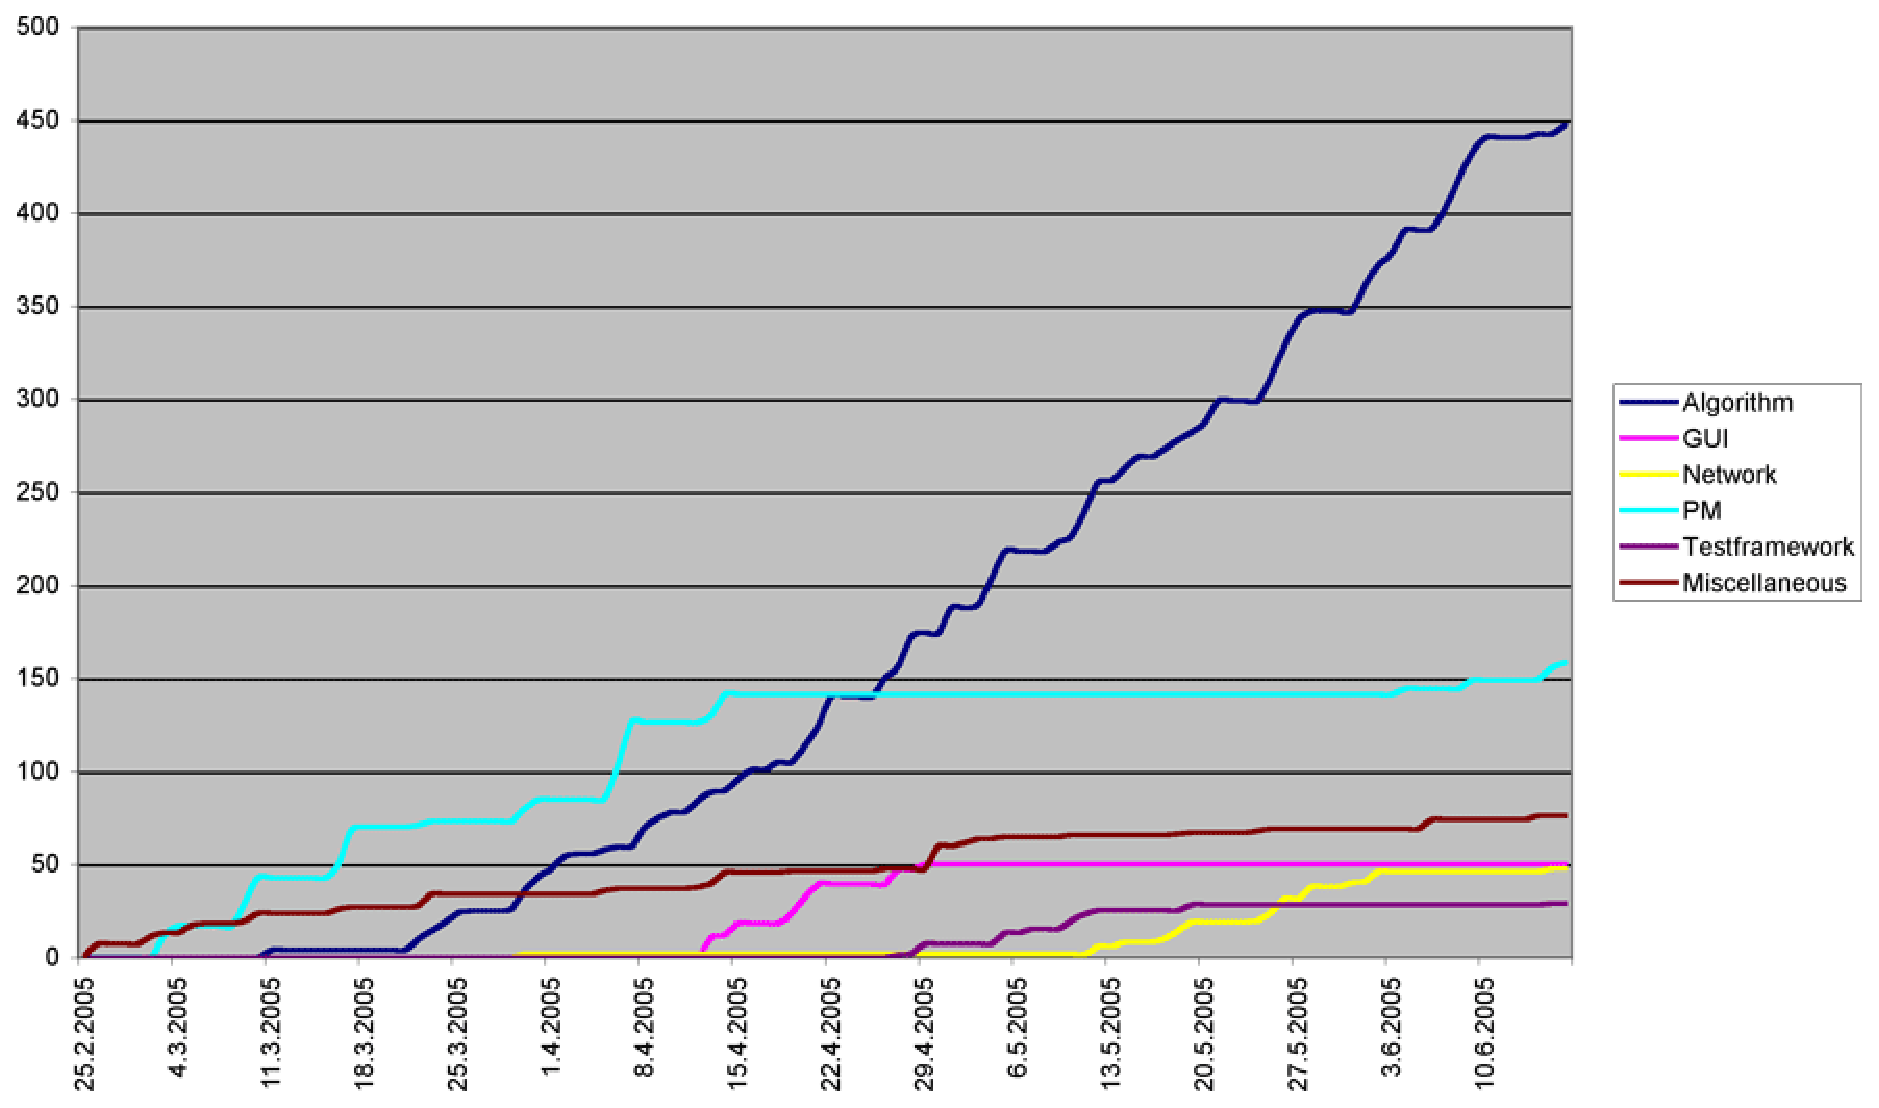
\includegraphics[height=10cm,width=15cm]{../../images/erfahrungsbericht/statistik1.eps}
%}
\caption{Arbeits-Fortschritt}
\label{Arbeits-Fortschritt}
\end{figure}


\newpage
\subsection{Modul-Statistiken}
Diese Statistik zeigt auf, an welchem Modul welche Aktivit�ten vorgenommen wurden. Beinahe die H�lfte der ganzen Arbeit wurde dem Modul Algorithmus zugeordnet.
\begin{figure}[H]
\centering
%\frame{
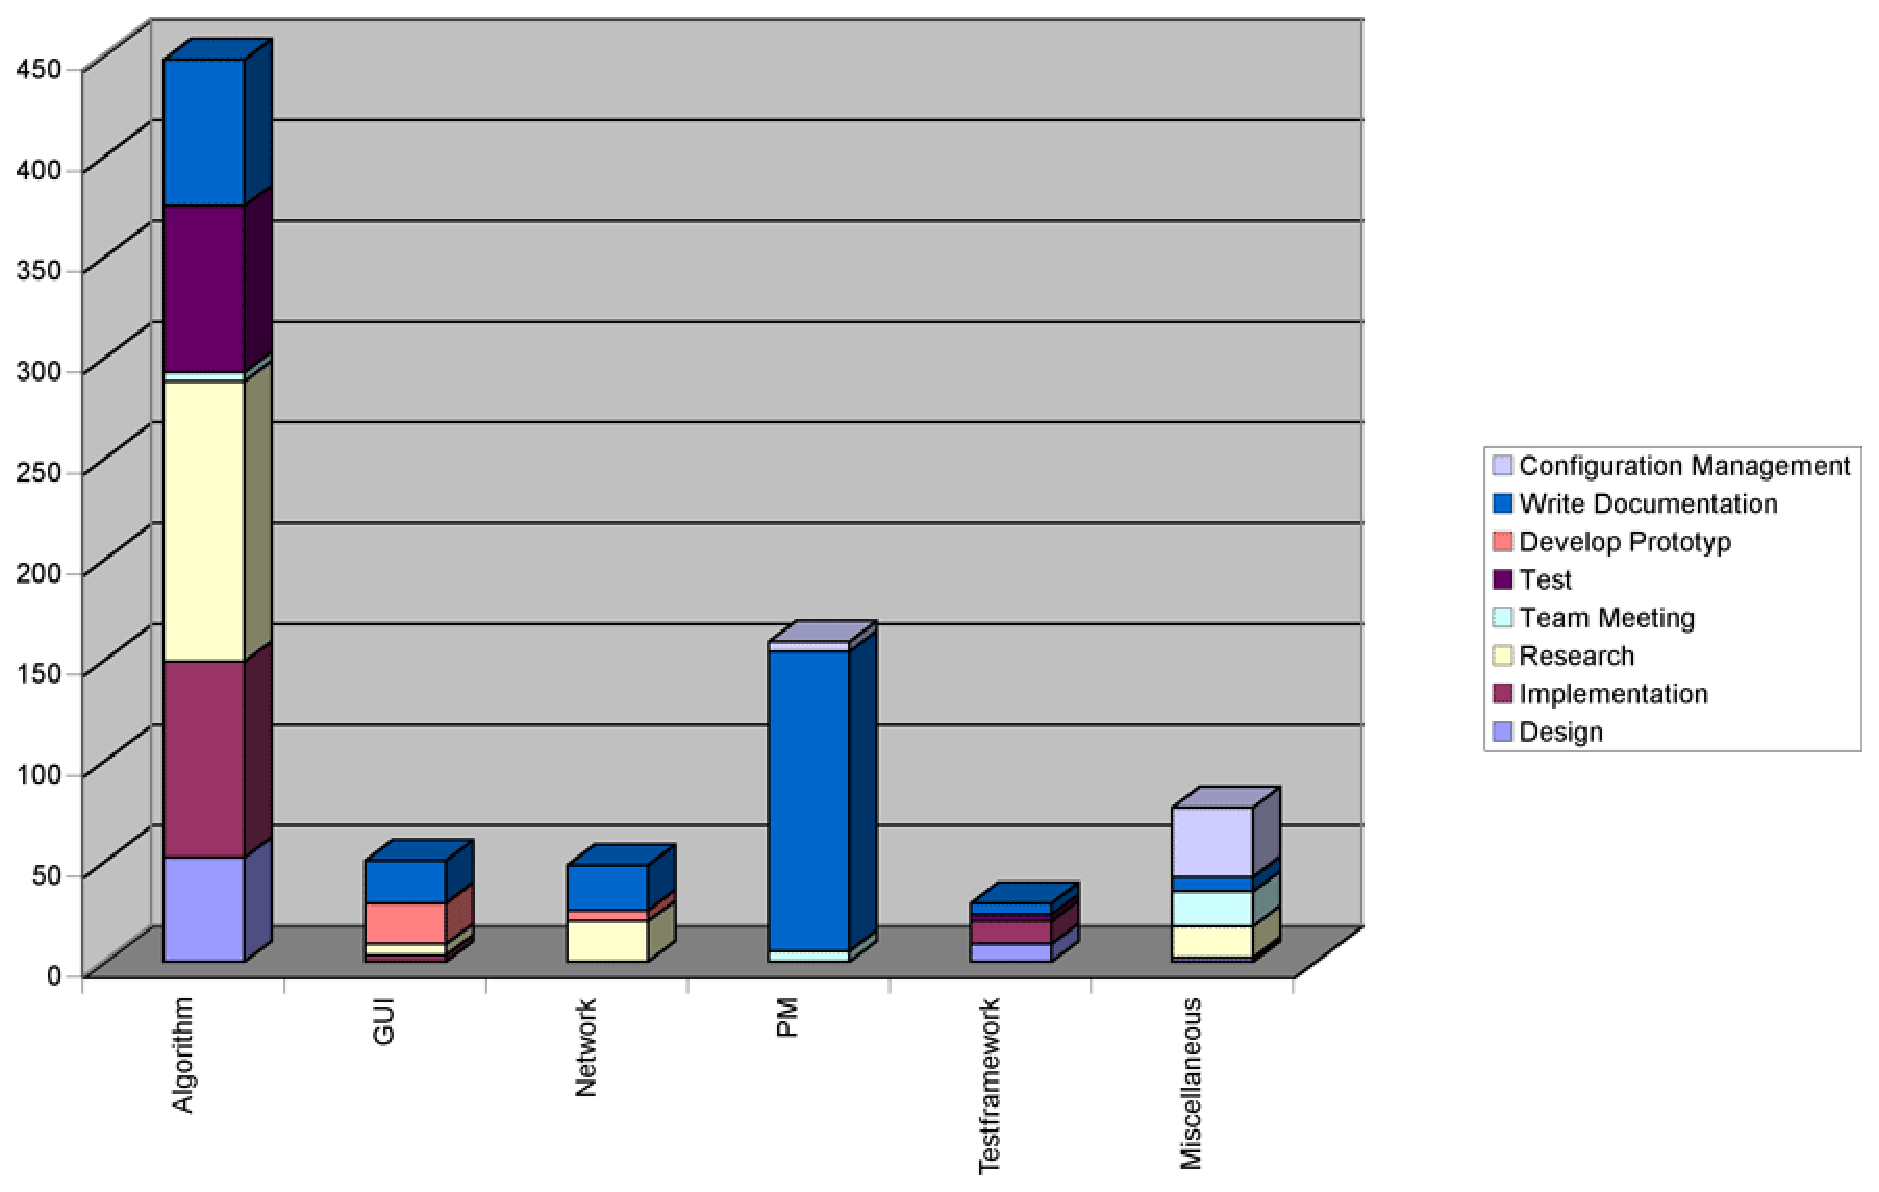
\includegraphics[height=10cm,width=15cm]{../../images/erfahrungsbericht/statistik3.eps}
%}
\caption{Modul-Statistiken}
\label{Modul-Statistiken}
\end{figure}


\newpage
\subsection{Aktivit�ten-Statistiken}
Anhand dieser Statistik ist zu sehen, welche Aktivit�ten f�r welche Module gemacht wurden. Allgemein ist deutlich ersichtlich, dass etwa ein Drittel unserer Aktivit�t aus dem Schreiben vom Dokumenten bestand. Ein grosser Teil davon f�r das Projektmanagement.
\begin{figure}[H]
\centering
%\frame{
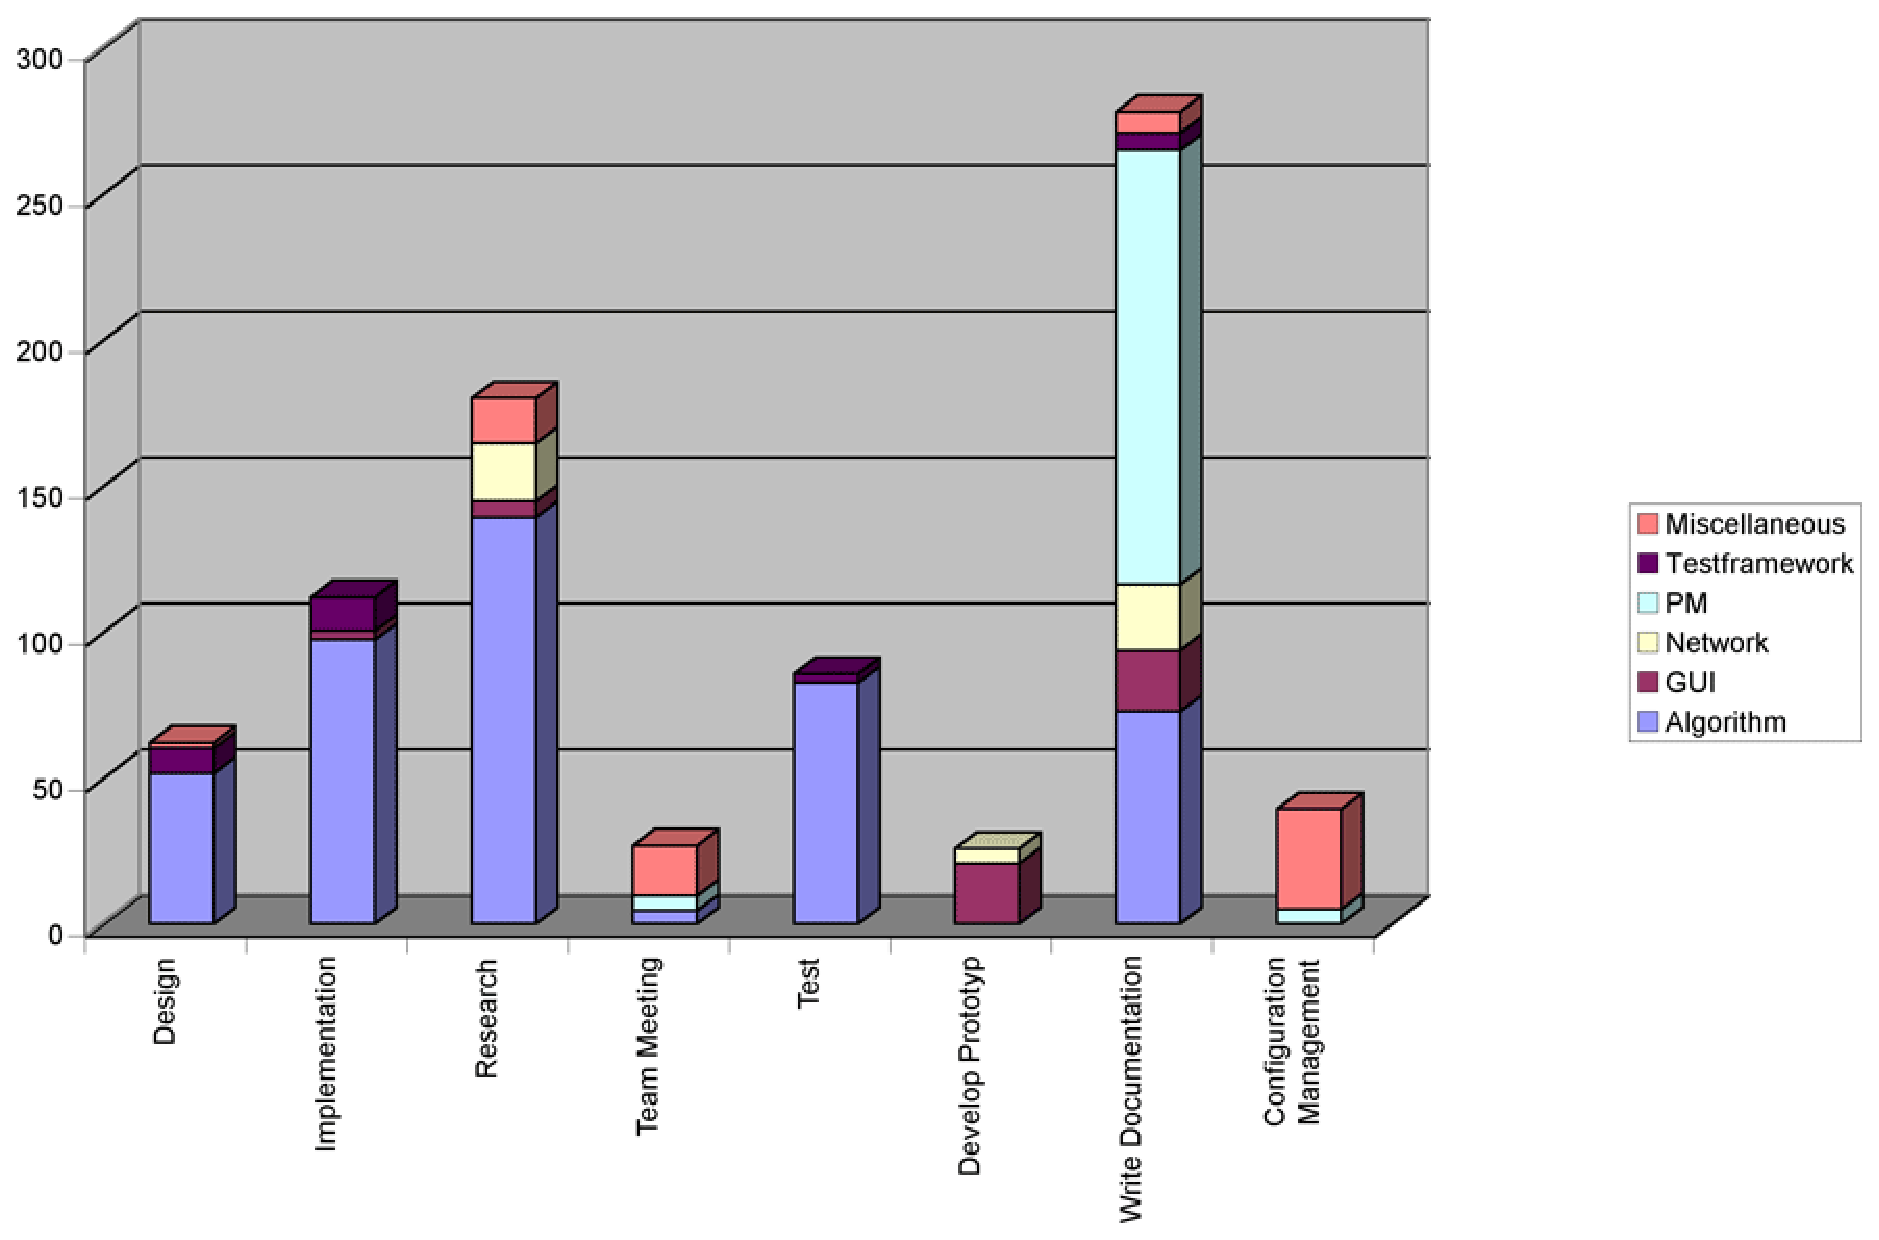
\includegraphics[height=10cm,width=15cm]{../../images/erfahrungsbericht/statistik4.eps}
%}
\caption{Aktivit�ten-Statistiken}
\label{Aktivit�ten-Statistiken}
\end{figure}